\section{Results and discussion}
\label{sec:results}

\subsection{Image-aware performance and shortcut controls}
The final answer distribution yields a strong task-majority baseline: the development-fitted task-majority rule attains 57.50\% (92/160). This result reflects the frozen answer distribution, particularly for count questions, without using visual evidence. The text-only S1\_LANGUAGE control reaches 28.75\% over 480 question--repeat instances, and the permitted-metadata S2\_METADATA control reaches 36.25\% (Table~\ref{tab:shortcut-controls}). Neither control receives imagery or detector evidence. In contrast, the image-aware A0\_NO\_RECHECK and T1\_TASK operating points reach 72.29\% and 75.00\%, respectively. Their paired gaps to S1 are $+43.54$ and $+46.25$ points, and to S2 are $+36.04$ and $+38.75$ points; all four 95\% ROI-cluster intervals exclude zero. The complete image-aware pipelines therefore outperform the evaluated controls based on question wording and permitted non-image metadata. Because S1/S2 also use a modality-specific prompt and omit the hybrid rule path, the comparison measures a pipeline-level difference and does not isolate the causal effect of image access.

\begin{table*}[!t]
\centering\small
\caption{Shortcut controls and image-aware operating points on the frozen final set. S0 uses a development-fitted task majority and is deterministic ($n=160$); all other rows use three aligned repeats ($n=480$). S1 receives question text, choices, and task type; S2 additionally receives permitted runtime metadata.}
\label{tab:shortcut-controls}
\resizebox{\textwidth}{!}{%
\begin{tabular}{lcccrrrrr}
\toprule
Method & Image & Detector evidence & Runtime metadata & Presence & Damage & Count & Spatial & Overall\\
\midrule
S0 task majority & no & no & task only & 68.18 & 65.91 & 65.12 & 17.24 & 57.50\\
S1 language only & no & no & question only & 31.82 & 34.09 & 32.56 & 10.34 & 28.75\\
S2 metadata only & no & no & permitted & 31.82 & 58.33 & 32.56 & 14.94 & 36.25\\
\midrule
A0\_NO\_RECHECK & yes & yes & permitted & 93.18 & 66.67 & 75.97 & 43.68 & 72.29\\
T1\_TASK & yes & yes & permitted & 93.18 & 75.76 & 78.29 & 41.38 & 75.00\\
\bottomrule
\end{tabular}}
\end{table*}

\subsection{Observation changes under matched answer calls}
The policy comparison alone cannot distinguish a new image from another answer opportunity. We therefore created paired branches at all 161 executed T1 rechecks, with each pair sharing its pre-recheck state. The fixed branch reran perception and answering on the previous view. The changed branch executed the original recheck before perception and answering. The strict validity gate accepted all 161 pairs, with no missing pair or execution error. The branch schedule reproduced the original recheck-step locations in 118 of 119 episodes; the one mismatch retained the same two rechecks but placed the second at a different step, reflecting re-runnable perception-path variation.

The changed-view branch produces correct candidate answers in 96/161 transitions (59.63\%), versus 81/161 (50.31\%) for the fixed-view matched call, a paired difference of $+9.32$ points (95\% ROI-cluster interval $[-2.00,+21.74]$). The point estimate is accompanied by 36 fixed-wrong/changed-correct transitions and 21 fixed-correct/changed-wrong transitions; 44 pairs are wrong in both branches and 60 correct in both. Answers disagree in 42.24\% of pairs. Thus the changed observation can alter the answer path beyond a repeated call on the old image, but the clustered interval does not establish a stable positive average effect in the sampled ROIs.

Excluding the one episode whose rerun placed its second recheck at step 2 rather than reference step 3 removes two wrong--wrong pairs. The remaining 159 pairs from 118 episodes have 81/159 fixed-view and 96/159 changed-view correct candidates, a $+9.43$-point paired difference (95\% ROI-cluster interval $[-2.03,+22.00]$), with the same 36 help and 21 harm transitions. As a separate old-view repeat check, the pre-recheck and fixed-branch image bytes and normalized candidate answers agree in all 161/161 original forks (159/159 after exclusion). The two old-view calls use different step seeds and evidence prompts, however, so this is observed answer stability under identical image bytes rather than a controlled same-prompt, same-seed repeatability estimate.

\begin{table}[htbp]
\centering\small
\caption{Fixed-view matched-call diagnostic at executed T1 recheck transitions. Candidate-answer correctness is measured immediately after the branch, not at episode termination. Presence has no T1 dedicated recheck.}
\label{tab:matched-view}
\begin{tabular}{lrrrrrr}
\toprule
Task & $n$ & Fixed & Changed & Help & Harm & $\Delta$ pp\\
\midrule
Damage & 123 & 46.34 & 58.54 & 27 & 12 & $+12.20$\\
Count & 18 & 83.33 & 100.00 & 3 & 0 & $+16.67$\\
Spatial & 20 & 45.00 & 30.00 & 6 & 9 & $-15.00$\\
\midrule
Overall & 161 & 50.31 & 59.63 & 36 & 21 & $+9.32$\\
\bottomrule
\end{tabular}
\end{table}

Figure~\ref{fig:help-harm-cases} grounds the aggregate transitions in two frozen T1 episodes. In the damage episode \nolinkurl{hurricane-michael_00000435_post_disaster__damage_0001_9430}, successive observations at approximately 1330, 887, and 443~m increase the marked building's predicted damage probability from 0.158 to 0.369 and 0.588. The answer consequently changes from the incorrect ``no damage'' to the correct ``damaged.'' This example illustrates the potential benefit of a more local observation for a damage question.

In contrast, the spatial episode \nolinkurl{hurricane-michael_00000306_post_disaster__spatial_0092_5452} shows the complementary risk. The wide observation selects a damaged building north of the ROI center and answers correctly. After descent, the evidence ranking selects a different building southwest of the center, changing a correct answer to an incorrect one. A further descent is rejected because predicted ROI coverage is 0.340, below the 0.98 gate. The failure involves a change in target identity under reduced regional context, rather than only bearing noise for a fixed target.

\begin{figure*}[!t]
\centering
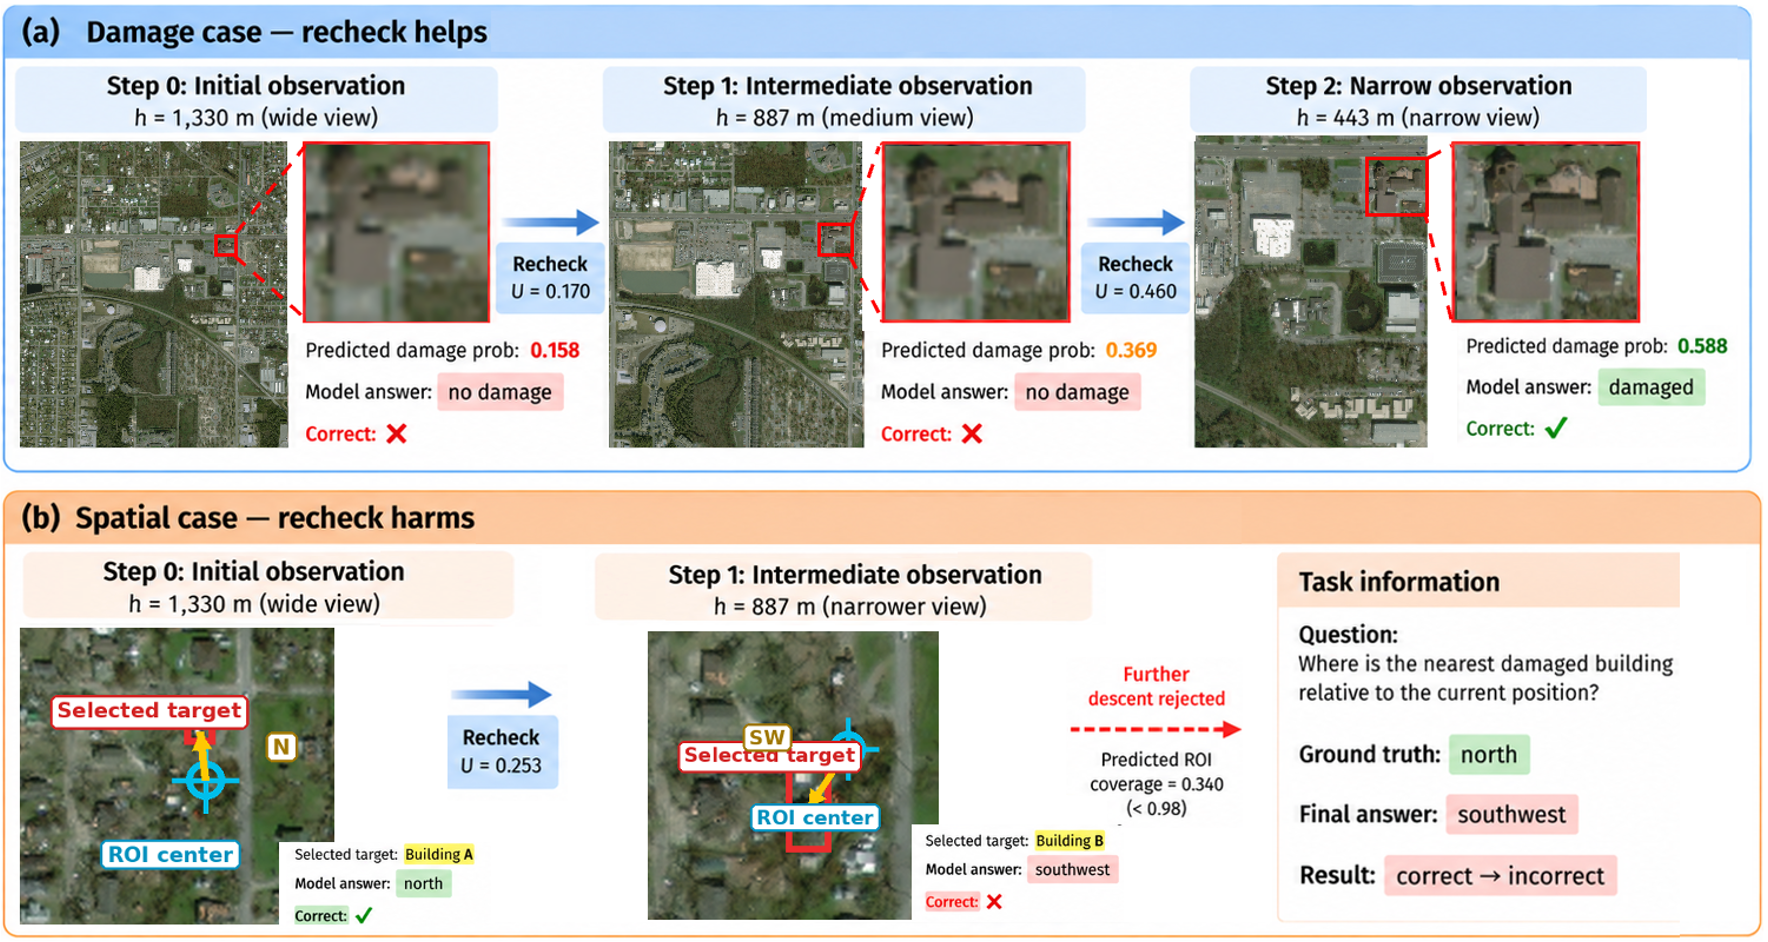
\includegraphics[width=\textwidth]{figure-paper/recheck成功失败两个案例.png}
\caption{Frozen examples of recheck help and harm. (a) Narrower observations strengthen evidence for a marked building and correct a damage answer. (b) A spatial recheck changes the selected nearest damaged building from the correct northern target to a southwestern target; the coverage gate then rejects further descent. The examples expose the action--observation--evidence--answer chain behind the aggregate help and harm counts.}
\label{fig:help-harm-cases}
\end{figure*}

\subsection{Building-level evidence and task-dependent outcomes}
The camera-ladder diagnostic holds 7,238 annotated buildings in 43 development ROIs fixed while changing the rendered footprint. ChangeOS localization recall rises from 22.09\% at cruise to 34.06\% at intermediate and 56.52\% at floor. With every unmatched ground-truth building counted as incorrect, binary building accuracy rises from 20.01\% to 31.06\% and 53.65\%. Among matched buildings only, binary damage accuracy is 90.56\%, 91.20\%, and 94.92\%, while matched-only macro-F1 is 0.8714, 0.8743, and 0.9232. The paired cruise-to-floor outcomes include 2,696 incorrect-to-correct changes and 261 correct-to-incorrect changes. The building-level diagnostic shows that rendering changes affect the predicted evidence available to the agent. Asymmetric pre-/post-image processing and changes in context prevent attributing these effects solely to GSD or physical descent.

Table~\ref{tab:detection-fp-audit} separates localization from conditional damage classification. Localization precision falls to 68.65\% at floor even as recall and matched-building damage accuracy rise; unmatched predictions increase to 43.44 per ROI. TP/FP/FN use a one-to-one nearest-centroid match within 12~m, so an unmatched prediction can reflect a duplicate, localization error, or missing annotation as well as a spurious building. The all-GT accuracy denominator includes missed buildings but does not penalize extra predictions; matched-only accuracy and macro-F1 exclude misses and unmatched predictions. The gains in damage accuracy and the increase in localization false positives thus describe different aspects of the detection pipeline.

\begin{table*}[!t]
\centering\small
\caption{ChangeOS localization and binary-damage audit on the same 43 development ROIs and 7,238 annotated buildings at each height. Loc. P/R are localization precision/recall; FP is an unmatched prediction, FN an unmatched GT building, and FP/ROI is FP/43. All-GT accuracy counts unmatched GT as wrong but does not count unmatched predictions; matched accuracy and macro-F1 condition on matched GT only.}
\label{tab:detection-fp-audit}
\resizebox{\textwidth}{!}{%
\begin{tabular}{lrrrrrrrrr}
\toprule
View (height) & TP & FP & FN & Loc. P (\%) & Loc. R (\%) & FP/ROI & All-GT acc. (\%) & Matched acc. (\%) & Matched macro-F1\\
\midrule
Cruise (1330 m) & 1,599 & 502 & 5,639 & 76.11 & 22.09 & 11.67 & 20.01 & 90.56 & 0.8714\\
Intermediate (887 m) & 2,465 & 677 & 4,773 & 78.45 & 34.06 & 15.74 & 31.06 & 91.20 & 0.8743\\
Floor (443 m) & 4,091 & 1,868 & 3,147 & 68.65 & 56.52 & 43.44 & 53.65 & 94.92 & 0.9232\\
\bottomrule
\end{tabular}}
\end{table*}

The matched-call results show that task answers also respond differently to observation changes. Damage and count transitions have positive point differences, whereas spatial transitions have a negative point difference (Table~\ref{tab:matched-view}). A more local view can improve the evidence for a marked building or a damaged-count decision, yet it can change the selected target for a nearest-building direction judgment. These task-wise estimates are descriptive because T1 selects the recheck subsets, which contain only 18 count and 20 spatial transitions.

\subsection{Complete-policy performance}
Table~\ref{tab:final-policies} reports the prespecified complete-policy runs. T1\_TASK has the highest observed terminal accuracy, 360/480 question--repeat instances (75.00\%), with 161 executed dedicated rechecks. A0\_NO\_RECHECK (the internal configuration identifier is A0\_HOLD) forbids dedicated rechecks but permits search and answers 347/480 (72.29\%). A2\_ALWAYS makes 923 rechecks and answers 307/480 (63.96\%). Active policies share a maximum of two dedicated rechecks. Their realized operating points differ in actions, model calls, and total cost, which are not matched in this comparison.

\begin{table}[htbp]
\centering\small
\caption{Primary frozen policy operating points on the same 160 questions under three generation repeats. Rechecks are executed dedicated actions and exclude search.}
\label{tab:final-policies}
\begin{tabular}{lrrr}
\toprule
Policy & Correct / 480 & Accuracy (\%) & Rechecks\\
\midrule
A0\_NO\_RECHECK & 347 & 72.29 & 0\\
A1\_RANDOM & 326 & 67.92 & 419\\
A2\_ALWAYS & 307 & 63.96 & 923\\
A3U\_RAW\_ENTROPY & 339 & 70.63 & 626\\
T1\_TASK & 360 & 75.00 & 161\\
\bottomrule
\end{tabular}
\end{table}

The 2.71-point T1\_TASK advantage over A0\_NO\_RECHECK is an observed difference of 13 correct question--repeat instances, not 13 distinct questions. Its 98.75\% multiplicity-adjusted interval includes zero (Table~\ref{tab:final-contrasts}), as does the comparison with raw entropy. The positive interval against A2\_ALWAYS supports a difference between these complete policies on the sampled ROIs; it does not show that T1's individual changed observations caused that difference.

\begin{table}[htbp]
\centering\small
\caption{Prespecified paired T1\_TASK terminal-accuracy contrasts in percentage points. The 98.75\% ROI-cluster intervals adjust for four comparisons.}
\label{tab:final-contrasts}
\begin{tabular}{lrr}
\toprule
Contrast & Difference & 98.75\% interval\\
\midrule
T1 minus A0\_NO\_RECHECK & $+2.71$ & $[-2.04,+7.50]$\\
T1 minus A1\_RANDOM & $+7.08$ & $[+0.01,+14.69]$\\
T1 minus A2\_ALWAYS & $+11.04$ & $[+0.86,+21.38]$\\
T1 minus A3U\_RAW\_ENTROPY & $+4.38$ & $[-4.33,+12.96]$\\
\bottomrule
\end{tabular}
\end{table}

At the terminal-episode level, presence is unchanged between T1 and A0\_NO\_RECHECK, damage and count are numerically higher for T1, and spatial accuracy is lower (Table~\ref{tab:shortcut-controls}). Performance also varies by event: T1 versus A0 is 54.86\% versus 58.33\% in Hurricane Michael, 84.31\% versus 77.12\% in Moore, and 83.06\% versus 79.23\% in Nepal. Together, the matched-call results and complete-policy comparisons characterize task-dependent corrections and harms. The interval for the A0 contrast and incomplete cost measurements limit conclusions about the overall effectiveness and efficiency of the recheck policy.
